\documentclass[11pt]{article}

\usepackage{
    amssymb,
    amsmath,
    amsfonts,
    calc,
    eurosym,
    geometry,
    ulem,
    graphicx,
    caption,
    color,
    setspace,
    sectsty,
    comment,
    footmisc,
    caption,
    % natbib,
    pdflscape,
    subcaption,
    subfiles,
    titling,
    array,
    hyperref,
    booktabs,
    longtable,
    float,
    authblk,
    makecell,
    threeparttable}


\usepackage[
    backend=biber,
    style=nature,
    date=year,
    doi=true,
    isbn=false,
    url=false,
    eprint=false
]{biblatex}

\AtEveryBibitem{%
  \clearfield{note}%
}
\AtEveryCitekey{\clearlist{publisher}}
\AtEveryBibitem{\clearlist{publisher}}

\usepackage{pgf,tikz}
\usetikzlibrary{arrows, automata}
\usetikzlibrary{shapes.geometric,positioning}
\usetikzlibrary{positioning,calc}

\usepackage{siunitx}
\newcolumntype{d}{S[input-symbols = ()]}

\normalem

\renewcommand\Affilfont{\small\itshape}

\onehalfspacing
\newtheorem{theorem}{Theorem}
\newtheorem{corollary}[theorem]{Corollary}
\newtheorem{proposition}{Proposition}
\newenvironment{proof}[1][Proof]{\noindent\textbf{#1.} }{\ \rule{0.5em}{0.5em}}

\newtheorem{hyp}{Hypothesis}
\newtheorem{subhyp}{Hypothesis}[hyp]
\renewcommand{\thesubhyp}{\thehyp\alph{subhyp}}

\newcommand{\red}[1]{{\color{red} #1}}
\newcommand{\blue}[1]{{\color{blue} #1}}

\newcolumntype{L}[1]{>{\raggedright\arraybackslash}m{#1}}
\newcolumntype{C}[1]{>{\centering\arraybackslash}m{#1}}
\newcolumntype{R}[1]{>{\raggedleft\arraybackslash}m{#1}}
\subsubsectionfont{\normalfont\itshape}

\usepackage{mathtools}

\usepackage{letltxmacro}
\LetLtxMacro\orgvdots\vdots
\LetLtxMacro\orgddots\ddots

\makeatletter
\DeclareRobustCommand\vdots{%
  \mathpalette\@vdots{}%
}
\newcommand*{\@vdots}[2]{%
  % #1: math style
  % #2: unused
  \sbox0{$#1\cdotp\cdotp\cdotp\m@th$}%
  \sbox2{$#1.\m@th$}%
  \vbox{%
    \dimen@=\wd0 %
    \advance\dimen@ -3\ht2 %
    \kern.5\dimen@
    % remove side bearings
    \dimen@=\wd2 %
    \advance\dimen@ -\ht2 %
    \dimen2=\wd0 %
    \advance\dimen2 -\dimen@
    \vbox to \dimen2{%
      \offinterlineskip
      \copy2 \vfill\copy2 \vfill\copy2 %
    }%
  }%
}
\DeclareRobustCommand\ddots{%
  \mathinner{%
    \mathpalette\@ddots{}%
    \mkern\thinmuskip
  }%
}
\newcommand*{\@ddots}[2]{%
  % #1: math style
  % #2: unused
  \sbox0{$#1\cdotp\cdotp\cdotp\m@th$}%
  \sbox2{$#1.\m@th$}%
  \vbox{%
    \dimen@=\wd0 %
    \advance\dimen@ -3\ht2 %
    \kern.5\dimen@
    % remove side bearings
    \dimen@=\wd2 %
    \advance\dimen@ -\ht2 %
    \dimen2=\wd0 %
    \advance\dimen2 -\dimen@
    \vbox to \dimen2{%
      \offinterlineskip
      \hbox{$#1\mathpunct{.}\m@th$}%
      \vfill
      \hbox{$#1\mathpunct{\kern\wd2}\mathpunct{.}\m@th$}%
      \vfill
      \hbox{$#1\mathpunct{\kern\wd2}\mathpunct{\kern\wd2}\mathpunct{.}\m@th$}%
    }%
  }%
}
\makeatother



\newcommand{\ode}[2]{\frac{d{#1}}{d{#2}}}

\geometry{left=1.0in,right=1.0in,top=1.0in,bottom=1.0in}

%\addbibresource{lipids.bib}

\begin{document}

% \begin{titlepage}
% \title{Estimating deaths averted due to vaccination using marginal structural models \thanks{abc}}
% \author[1]{Christopher Boyer\thanks{email: \href{mailto:cboyer@g.harvard.edu}{cboyer@g.harvard.edu}}}
% \author[1]{Marc Lipsitch}
% \affil[1]{Department of Epidemiology, Harvard T.H. Chan School of Public Health, Boston, MA.}
% \date{\today}
% \maketitle

% \begin{abstract}
% \noindent \\
% \vspace{0in} \\
% \noindent\textbf{Keywords:} target trial, vaccines, immortal time bias, effectiveness, monkeypox, postexposure prophylaxis, infectious disease \\

% \bigskip
% \end{abstract}
% \setcounter{page}{0}
% \thispagestyle{empty}
% \end{titlepage}
% \pagebreak \newpage

% \doublespacing

% \section{Introduction} \label{sec:introduction}




Consider the following compartmental model waning natural immunity, death, and a waning vaccine with partial effectiveness against infection and death.
\begin{align}
    \begin{split}\label{eqn:sirv}
    \ode{S_t}{t} &=  - \frac{\beta S_t (I^s_t + I^v_t)}{N} + \omega R_t - \nu S_t + \sigma V_t \\
    \ode{I^s_t}{t} &=  \frac{\beta S_t (I^s_t + I^v_t)}{N} - \gamma_s I^s_t \\
    \ode{I^v_t}{t} &=  (1 - \theta) \frac{\beta V_t (I^s_t + I^v_t)}{N} - \gamma_v I^v_t  \\
    \ode{R_t}{t} &=  (1 - \mu_s) \gamma I^s_t +(1 - \mu_v) \gamma I^v_t - \omega R_t \\
    \ode{V_t}{t} &=  \nu S_t - (1 - \theta) \frac{\beta V_t (I^s_t + I^v_t)}{N}  - \sigma V_t \\
    \ode{D^s_t}{t} &=  \mu_s \gamma_s I^s_t \\
    \ode{D^v_t}{t} &=  \mu_v \gamma_v I^v_t
    \end{split}
\end{align}
where $N$ is population size, $S_t$ is the number of susceptibles, $I^s_t$ is the number of naturally infections, $I^v_t$ is the number of vaccine breakthrough infections, $R_t$ are the recovered (due to infection), $V_t$ are the vaccinated, and $D^s_t$ and $D^v_t$ are deaths among the vaccinated and unvaccinated at time $t$. 

\begin{table}[h]
    \centering
    \caption{Chosen parameter values for compartmental model}
    \begin{tabular}{|c|c|l|}
        \hline
        Parameter & Value & Description \\
        \hline
        $S_0$ & 10000 & initial susceptibles \\
        $I_0$ & 1 & initial infected \\
        $\beta$ & 0.3&   infection rate \\
        $\gamma_s$ & 0.08&   recovery rate \\
        $\gamma_v$ & 0.08&   recovery rate for breakthroughs \\
        $\mu_s$ & 0.1&   CFR \\
        $\mu_v$ & 0.005&   CFR for breakthroughs \\
        $\omega$ & 0.005& rate of waning natural immunity \\
        $\sigma$ & 0.01& rate of waning vaccine immunity  \\
        $\nu$ & varied & vaccination rate  \\
        $\theta$ & 0.5&  vaccine efficacy against infection \\
        \hline
    \end{tabular}
\end{table}


\begin{figure}[t]
    \centering
    \begin{tikzpicture}[> = stealth, shorten > = 1pt, auto, node distance = 3.5cm, thick]
    
    \node[circle,draw] (r) {$R_t$};
    \node[circle,draw] (is) [above left of=r] {$I_t^s$};
    \node[circle,draw] (iv) [below left of=r] {$I_t^v$};
    \node[circle,draw] (s) [left of=is] {$S_t$};
    \node[circle,draw] (v) [left of=iv] {$V_t$};
    \node[circle,draw] (ds) [above right of=r] {$D_t^s$};
    \node[circle,draw] (dv) [below right of=r] {$D_t^v$};


    \path[->] (s) edge node {$\frac{\beta (I^s_t + I^v_t)}{N}$} (is);
    \path[->] (is) edge node {$(1-\mu_s) \gamma_s$} (r);
    \path[->] (iv) edge node {$(1-\mu_v) \gamma_v$} (r);
    \path[->] (is) edge node {$\mu_s \gamma_s$} (ds);
    \path[->] (iv) edge node {$\mu_v \gamma_v$} (dv);
    \path[->] (r) edge node {$\omega$} (s);
    \path[->] (v) edge node {$(1-\theta)\frac{\beta (I^s_t + I^v_t)}{N}$} (iv);
    \path[->] (v) edge node {$\sigma$} (s);


    \end{tikzpicture}
   
    \caption{Compartmental model with waning natural immunity, death, and a waning vaccine with partial effectiveness against infection and death.}
    \label{fig:design1}
    \end{figure}

    \begin{figure}[b]
        \centering
        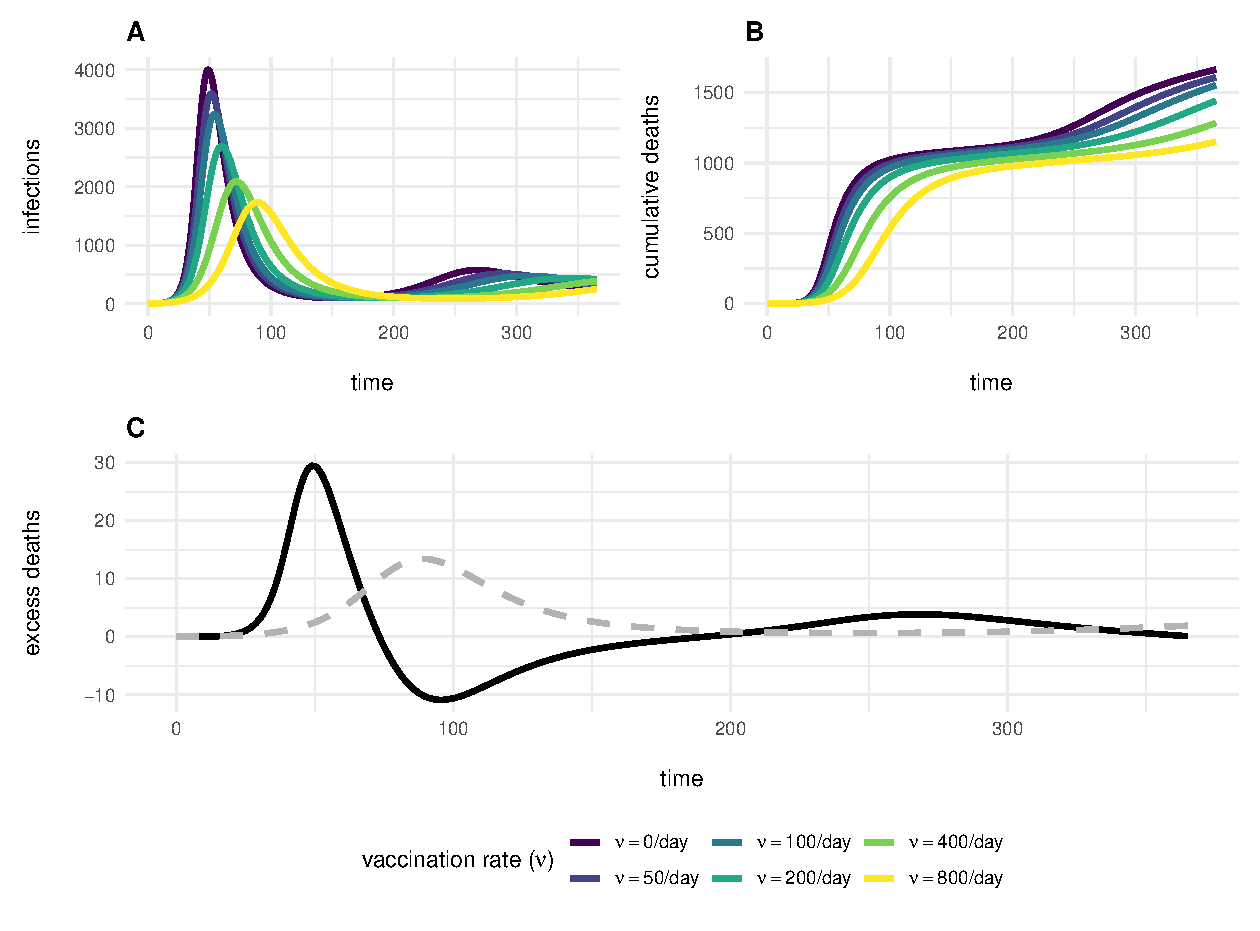
\includegraphics[width=\linewidth]{../3_figures/deaths_averted.pdf}
        \caption{Modeled infections (A), cumulative deaths (B), and excess deaths (C) under different vaccination regimes. In panel C we compare 800/day to 0/day strategies and calculate excess deaths using the naive method (dotted line) and modeled differences (solid line).}
    \end{figure}

    \begin{figure}[t]
        \centering
        \begin{tikzpicture}[> = stealth, shorten > = 1pt, auto, node distance = 1.75cm, thick]
        
        \node[circle,draw=none] (v0) {$V_{t-\delta}$};
        \node[circle,draw=none] (s0) [below of=v0] {$S_{t-1}$};
        \node[circle,draw=none] (i0) [right of=s0] {$I_{t-1}$};
        \node[circle,draw=none] (r0) [right of=i0] {$R_{t-1}$};
        \node[circle,draw=none] (d0) [below of=r0] {$D_{t-1}$};
        \node[circle,draw=none] (s) [right of=r0] {$S_t$};
        \node[circle,draw=none] (v) [above of=s] {$V_t$};
        \node[circle,draw=none] (i) [right of=s] {$I_t$};
        \node[circle,draw=none] (r) [right of=i]  {$R_t$};
        \node[circle,draw=none] (d) [below of=r] {$D_t$};    
    
        \path[->] (s0) edge node {} (i0);
        \path[->] (i0) edge node {} (r0);
        \path[->] (r0) edge node {} (s);
        \path[->] (s0) edge node {} (i0);
        \path[->] (s0) edge [out=30, in=150] node {} (s);
        \path[->] (s0) edge [out=30, in=180] node {} (v);
        \path[->] (v0) edge node {} (i);
        \path[->] (v0) edge node {} (d);

        \end{tikzpicture}
       
        \caption{Compartmental model with waning natural immunity, death, and a waning vaccine with partial effectiveness against infection and death.}
        \label{fig:design1}
        \end{figure}
% Solving the second equation conditional on $S_t$ and $V_t$ yields $I_t = I_{t-1}\operatorname{exp}\{\int_{t-1}^t\beta S_u/N + (1 - \theta) \beta V_u/N - \gamma + \epsilon  \,du\}$ which can be discretized as 
% \begin{equation}\label{eqn:discrete}
%     I_t \approx I_{t-1}\operatorname{exp}\left\{\frac{\beta S_t}{N} + (1 - \theta) \frac{\beta V_t}{N} - \gamma + \epsilon \right\}
% \end{equation}
% when $S_u \approx S_t$ for all $u \in (t-1, t)$. This implies, even for this relatively simple model, the number of infections is a function of the fraction of susceptibles and the fraction of vaccinated, both of which can vary over time (e.g. due to waning immunity from natural infection and vaccination).  

% Equations \ref{eqn:sirv} and \ref{eqn:discrete} suggest the following structural equation models
% \begin{align*}
%     A_t &= f(\overline{L}_t, \overline{A}_{t-1}, \overline{I}_{t-1}, \overline{Y}_{t-1}, \xi_{A_t})\\
%     I_t &= I_{t-1}\operatorname{exp}\{c_t + \zeta(A_t)\} + \xi_{I_t} \\
%     Y_t &= \sum_{s=1}^t p(s, t)I_s (1 - A_s) + q(s, t) I_s A_s + \xi_{Y_t}
% \end{align*}
% where our treatment is vaccination rate $A_t = \nu(t)$ and our outcome is number of deaths $Y_t$ at time $t$. Here $\xi_{A_t}$, $\xi_{I_t}$, and $\xi_{Y_t}$ are mean-zero random variables and $p(s, t)$ denotes the probability that someone infected at time $s$ dies due to infection at $t$. The second equation has the form of \ref{eqn:discrete}, but here $c_t$ collapses time-varying changes in susceptibility, recovery, and importation of infections and $\zeta(A_t)$ is the effect of . Applying the g-formula yields
\clearpage
\newpage
$$
E[Y_t^{\overline{a}_t} \mid X] = \sum_{s=1}^t p(s, t) \operatorname{exp}\left\{c_0(s) + \sum_{r=1}^s \zeta(A_t) - \sum_{r=1}^s \lambda(A_t)\right\}
$$


$$
E[Y_t^{\overline{a}_t} \mid X = x] = \operatorname{expit}\left\{\lambda(t,x) + \alpha_x \sum_{s=1}^{t}A_sI(X = x) + \beta_x \sum_{s=1}^{t-\delta}A_sI(X = x) \right\}
$$

$$
W = \frac{f(A_t \mid \overline{A}_{t-1})}{f(A_t \mid \overline{L}_t, \overline{A}_{t-1}, \overline{Y}_{t-1})}
$$



\begin{align}
    \begin{split}\label{eqn:sirv}
    \ode{S_t}{t} &=  - \frac{\beta S_t I_t}{N} + \omega R_t - \nu S_t + \sigma V_t \\
    \ode{I_t}{t} &=  \frac{\beta S_tI_t}{N} + (1 - \theta) \frac{\beta V_t I_t}{N} - \gamma I_t \\
    \ode{R_t}{t} &=  (1 - \mu) \gamma I_t - \omega R_t \\
    \ode{V_t}{t} &=  \nu S_t - (1 - \theta) \frac{\beta V_t I_t}{N}  - \sigma V_t \\
    \ode{D_t}{t} &=  \mu \gamma I_t \\
    \end{split}
\end{align}


% \begin{equation}\label{eqn:discrete2}
%     I_t \approx I_{t-1}\operatorname{exp}\left\{\frac{\beta}{N}S_{t-1}\exp\{ - \frac{\beta I_t}{N} + \omega R_t - \nu(t) + \sigma V_t\} + (1 - \theta) \frac{\beta}{N}V_{t-1}\exp\{\nu(t) S_t - (1 - \theta) \frac{\beta I_t}{N}  - \sigma\} - \gamma + \epsilon \right\}
% \end{equation}


% \begin{align}
%     \begin{split}\label{eqn:sirv}
%     \ode{S_t}{t} &=  - \frac{\beta S_t I_t}{N} + \omega R_t - \nu(t) S_t \\
%     \ode{I_t}{t} &=  \frac{\beta S_t I_t}{N} - \gamma I_t + \epsilon \\
%     \ode{R_t}{t} &=  \gamma I_t - \omega R_t
%     \end{split}
% \end{align}

% \begin{align*}
%     \ode{S_t}{t} &=  - \frac{\beta S_t I_t}{N} + \omega R_t - \nu S_t + \sigma V_t \\
%     \ode{E_t}{t} &=  \frac{\beta S_t I_t}{N} + (1 - \theta) \frac{\beta V_t I_t}{N} - \delta E_t + \epsilon \\
%     \ode{I_t}{t} &=  \delta E_t - \gamma (1 - \mu) I_t - \rho \mu I_t \\
%     \ode{R_t}{t} &=  \gamma (1 - \mu) I_t - \omega R_t \\
%     \ode{V_t}{t} &=  \nu S_t - (1 - \theta) \frac{\beta V_t I_t}{N}  - \sigma V_t \\
%     \ode{D_t}{t} &=  \rho \mu I_t\\
% \end{align*}
% %\printbibliography

% \subfile{supplement.tex}

% \onehalfspacing

\end{document}